\section{x86}

\subsection{MSVC}

\RU{Рассмотрим пример, скомпилированный в}\EN{Here is what we get after compilation} (MSVC 2010 Express):

\lstinputlisting[label=src:passing_arguments_ex_MSVC_cdecl,caption=MSVC 2010 Express]{patterns/05_passing_arguments/msvc.asm.\LANG}

\index{x86!\Registers!EBP}
\RU{Итак, здесь видно: в функции \main заталкиваются три числа в стек и вызывается 
функция \TT{f(int,int,int)}.}
\EN{What we see is that the \main function pushes 3 numbers onto the stack and calls \TT{f(int,int,int).}} 
\RU{Внутри \ttf доступ к аргументам, также как и к локальным переменным, происходит через макросы: 
\TT{\_a\$ = 8}, но разница в том, что эти смещения со знаком \IT{плюс}, 
таким образом если прибавить макрос \TT{\_a\$} к указателю на \EBP, то адресуется \IT{внешняя} 
часть \glslink{stack frame}{фрейма} стека относительно \EBP.}
\EN{Argument access inside \ttf is organized with the help of macros like: \TT{\_a\$ = 8}, 
in the same way as local variables,
but with positive offsets
(addressed with \IT{plus}).
So, we are addressing the \IT{outer} side of the \gls{stack frame} by adding the \TT{\_a\$} macro to the value in the \EBP register.}

\index{x86!\Instructions!IMUL}
\index{x86!\Instructions!ADD}
\RU{Далее всё более-менее просто: значение $a$ помещается в \EAX. 
Далее \EAX умножается при помощи инструкции \IMUL на то, что лежит в \TT{\_b}, 
и в \EAX остается \glslink{product}{произведение} этих двух значений.}
\EN{Then the value of $a$ is stored into \EAX. After \IMUL instruction execution, the value in \EAX is 
a \gls{product} of the value in \EAX and the content of \TT{\_b}.}
\RU{Далее к регистру \EAX прибавляется то, что лежит в \TT{\_c}.}
\EN{After that, \ADD adds the value in \TT{\_c} to \EAX.}
\RU{Значение из \EAX никуда не нужно перекладывать, оно уже лежит где надо. 
Возвращаем управление вызываемой функции~--- она возьмет значение из \EAX и отправит его в \printf.}
\EN{The value in \EAX does not need to be moved: it is already where it must be.
On returning to \gls{caller}, it takes the \EAX value and use it as an argument to \printf.}

\ifdefined\IncludeOlly
\subsection{MSVC + \olly}
\index{\olly}
\RU{Проиллюстрируем всё это в}\EN{Let's illustrate this in} \olly.
\RU{Когда мы протрассируем до первой инструкции в \ttf, которая использует какой-то из аргументов
(первый), мы увидим, что \EBP указывает на \glslink{stack frame}{фрейм стека}, 
я выделил его красным прямоугольником.}
\EN{When we trace to the first instruction in \ttf that uses one of the arguments 
(first one), we see that \EBP is pointing to the \gls{stack frame}, 
which I marked with a red rectangle.}
\RU{Самый первый элемент \glslink{stack frame}{фрейма стека} --- это сохраненное значение \EBP, 
затем \ac{RA}, третий элемент это
первый аргумент функции, затем второй аргумент и третий}\EN{The first element of the \gls{stack frame} is the saved value of \EBP, 
the second one is \ac{RA}, the third is the first function argument, then the second and third ones}.
\RU{Для доступа к первому аргументу функции, нужно прибавить к \EBP аккурат 8 (2 32-битных слова)}
\EN{To access the first function argument, one needs to add exactly 8 (2 32-bit words) to \EBP}.

\olly \EN{is aware about this, so it has added comments to the stack elements like}
\RU{в курсе этого, так что он добавил комментарии к элементам стека вроде}
``RETURN from'' \AndENRU ``Arg1 = \dots'', \EN{etc.}\RU{и т.д.}

N.B.: \EN{Function arguments are not members of the function's stack frame, they are rather
members of the stack frame of the \gls{caller} function.}
\RU{аргументы функции являются членами фрейма стека вызывающей функции а не текущей.}
\EN{Hence, \olly marked ``Arg'' elements as members of another stack frame.}
\RU{Поэтому \olly отметила элементы ``Arg'' как члены другого фрейма стека.}

\begin{figure}[H]
\centering
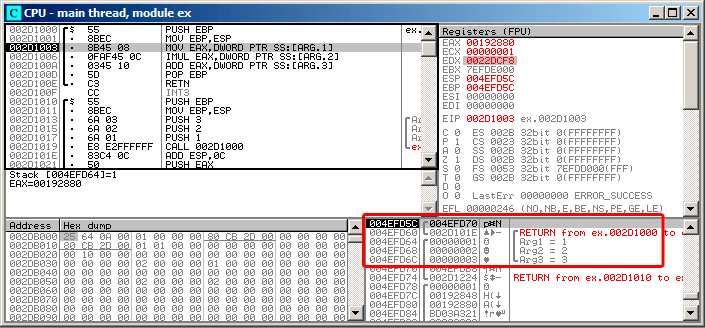
\includegraphics[scale=\FigScale]{patterns/05_passing_arguments/olly.png}
\caption{\olly: \RU{внутри функции}\EN{inside of} \ttf{}\EN{ function}}
\label{fig:passing_arguments_olly}
\end{figure}

\fi

\ifdefined\IncludeGCC
\subsection{GCC}

\RU{Скомпилируем то же в GCC 4.4.1 и посмотрим результат в \IDA:}
\EN{Let's compile the same in GCC 4.4.1 and see the results in \IDA:}

\lstinputlisting[caption=GCC 4.4.1]{patterns/05_passing_arguments/gcc.asm.\LANG}

\RU{Практически то же самое, если не считать мелких отличий описанных ранее.}
\EN{The result is almost the same with some minor differences discussed earlier.}

\RU{После вызова обоих функций \glslink{stack pointer}{указатель стека} не возвращается назад, 
потому что предпоследняя инструкция}
\EN{The \gls{stack pointer} is not set back after the two function calls(f and printf), 
because the penultimate} \TT{LEAVE} (\myref{x86_ins:LEAVE}) 
\RU{делает это за один раз, в конце исполнения.}
\EN{instruction takes care of this at the end.}
\fi
